\section{\trMorseLemma{}与\trCriticalPoint{}的\trIndex}
\label{sec:the-morse-lemma-index}\BookIndexDefinition{trIndex}

现在，让我们来描述一个\trMorseFunction{}的\trCriticalPoint{}附近会发生些什么。

\subsection{\trMorseLemma}
\label{subsec:the-morse-lemma}

在一个\trCriticalPoint{}的邻域内，函数会被它的二阶导数（的一半）十分贴近地逼近。\trMorseLemma{}给出的结果要好得多：必要时换一张\trChart，二者就相等了。

\begin{theorem}[\trMorseLemma]\label{thm:morse-lemma}\BookIndexDefinition{trMorseChart}\BookIndexDefinition{trMorseLemma}
设 $c$ 是函数 $f\colon V\to\RR$ 的一个\trNondegenerate\trCriticalPoint。那么，存在 $c$ 的一个邻域 $U$ 与一个\trDiffeomorphism{} $\varphi\colon(U,c)\to(\RR^n,0)$，使得
\[
f\circ\varphi^{-1}(x_1,\dotsc,x_n)
  =f(c)-\sum_{j=1}^{i}x_j^2+\sum_{j=i+1}^{n}x_j^2\text{。}
\]
\end{theorem}

\begin{proof}
这个结果也可以借\trHadamard{}引理来证明，\trMilnor{}在 [54] 中正是这样做的。我们在此选用的证明，则是\textbf{\trImplicitFunctionTheorem}（implicit function theorem）的一个直接应用，可在 [47] 中找到。\footnote{这个证明的主要优点，是它能给出比\trMorseLemma{}稍微更一般的结果：在\trCriticalPoint{}附近，一个函数可以写成一个常数、一个\trRank{}为~$k\leq n$ 的\trQuadraticForm{}以及一个其余 $n-k$ 个变量的函数三者之和，最后这个函数在所论点处的一阶与二阶偏导数全都为零。}

由于结果是局部性的，借助于一张\trChart，我们可以——而且我们也就是这样做的——假定 $V=\RR^n$、\trCriticalPoint{} $c$ 为 $0$。再通过与\trVectorSpace{}的一个\trIsomorphism{}作复合，我们进而还可以——而且也确实这样做了——假定\trQuadraticForm{} $(d^2f)_0$ 是对角的。

我们将按维数作归纳来证明这个结果。先从 $n=1$ 的情形开始，此时
\[
\begin{aligned}
f(x)&=f(0)+\frac{1}{2}f''(0)x^2+\varepsilon(x)x^2\\
&=f(0)\pm a\,x^2\bigl(1+\varepsilon(x)\bigr)
\end{aligned}
\]
其中 $a$ 为一个正实数，$\varepsilon$ 为一个 $\cC^\infty$ 函数，即
\[
\varepsilon(x)=\frac{1}{2}\int_0^x f^{(3)}(t)\,(x-t)^2\,dt\text{。}
\]
\footnote{译注：按所给积分，$\varepsilon$ 是三阶余项本身，须再除以 $x^{2}$ 才是首式中的余项系数（取 $f=x^{2}+x^{3}$ 即见首式不成立）；证明仍可自救：设 $b=\frac{1}{2}f''(0)\neq 0$、$r=R/x^{2}$（$R$ 为三阶余项，$r$ 在 $0$ 处\trSmooth{}延拓）、$\eta=r/b$，则 $f=f(0)+bx^{2}(1+\eta)$，取坐标 $x_{1}=x\sqrt{|b|\,(1+\eta)}$ 仍可完成证明。此处照原书排印，存疑备案。——译者注}
我们令
\[
x_1=\varphi(x)=x\sqrt{a\bigl(1+\varepsilon(x)\bigr)}\text{。}
\]
显然，$\varphi$ 是一个局部\trDiffeomorphism（因为 $\varphi'(0)=\sqrt{a}\neq 0$），这使我们得以应用\textbf{\trLocalInversionTheorem}（local inversion theorem），于是在 $0$ 的邻域内便有
\[
f\circ\varphi^{-1}(x_1)=f(x)=f(0)\pm x_1^2\text{。}
\]
这便是 $n=1$ 情形下的定理。

接下来，我们把 $\RR^n$ 写成 $\RR\times\RR^{n-1}$，并将其中的点记作 $(x,y)$。我们记 $f(x,y)=f_y(x)$，也就是把诸函数 $f_y$ 视为一个实变元的函数，而让参数 $y$ 在 $\RR^{n-1}$ 中变动。$f$ 的二阶\trTaylor{}多项式便是
\[
f(x,y)=f_y(0)+f'_y(0)\,x+\frac{1}{2}f''_y(0)\,x^2+x^2\varepsilon(x,y)\text{。}
\]
若 $f'_y(0)$ 这一项为零，那么我们便照 $n=1$ 的情形进行，因为 $f''_y(0)\neq 0$（否则 $f$ 的二阶导数矩阵中就会出现一个零列），这使得我们能够写出
\[
f(x,y)=f_y(0)\pm a(y)\,x^2\bigl(1+\varepsilon(x,y)\bigr)\text{，其中 }a(y)>0\text{。}
\]
映射
\[
\varphi\colon(x,y)\longmapsto
  \bigl(x_1=x\sqrt{a(y)\bigl(1+\varepsilon(x,y)\bigr)},\ y_1=y\bigr)
\]
正如 $n=1$ 的情形那样是一个局部\trDiffeomorphism，并且再同那一情形一样，它给出
\[
f\circ\varphi^{-1}(x_1,y_1)=\pm x_1^2+f(0,y_1)\text{，}
\]
从而使我们能够归纳地得出结论。

因此，让我们来证明：可以化归到 $f'_y(0)=0$ 的情形。让我们求出 $f_y$ 的诸\trCriticalPoint，即方程
\[
\frac{\partial f}{\partial x}(x,y)=0\text{。}
\]
的解。在关于 $(d^2f)_0$ 的假设下，我们知道
\[
\frac{\partial^2 f}{\partial x^2}(0,0)\neq 0\text{，}
\]
于是\trImplicitFunctionTheorem{}便断言：在 $(0,0)$ 的邻域内，我们的解正是某个函数 $\varphi$ 的图像 $x=\varphi(y)$ 上的那些点，这个 $\varphi$ 在 $0\in\RR^{n-1}$ 的邻域内有定义且属于 $\cC^\infty$ 类。既然我们已经假定二阶导数是对角的，$\partial f/\partial x$ 关于变量 $y$ 的导数在 $(0,0)$ 处就为零。于是，$(d\varphi)_0=0$。

现在我们使用（在 $0$ 邻域内的）局部\trDiffeomorphism{} $\boldsymbol{\Phi}(x,y)=(x+\varphi(y),\,y)$，它在 $0$ 处的\trDifferential{}是恒等映射。函数 $f\circ\boldsymbol{\Phi}$ 满足
\[
\left\{
\begin{array}{l}
\dfrac{\partial}{\partial x}(f\circ\boldsymbol{\Phi})(0,y)=0\\[2ex]
d^2(f\circ\boldsymbol{\Phi})_{(0,0)}=(d^2f)_{(0,0)}\text{。}
\end{array}
\right.
\]
把这个局部\trDiffeomorphism{} $\boldsymbol{\Phi}$ 吸收进记号之中——也就是说，对函数 $f\circ\boldsymbol{\Phi}$ 依旧使用记号 $f$——我们就化归到了具有所需性质的函数的情形。\trMorseLemma{}的证明至此结束。
\end{proof}

\trMorseLemma{}所给出的坐标在其开集内有定义的那种\trChart，就称为一个\textbf{\trMorseChart}（Morse chart）。

\trMorseLemma{}的一个直接推论是下述结果（另见\cref{ex:ch01-02}）。

\begin{corollary}\label{thm:nondegenerate-critical-isolated}
一个函数的诸\trNondegenerate\trCriticalPoint{}都是\textbf{\trIsolated}（isolated）{}的。\noqed
\end{corollary}

特别地，\trCompact\trManifold{}上的一个\trMorseFunction{}只有有限多个\trCriticalPoint。

\trMorseLemma{}的陈述中出现的整数 $i$，就是这个\trCriticalPoint{}的\trIndex（它只依赖于该\trCriticalPoint{}本身；$(n-i,\,i)$ 就是二阶导数\trQuadraticForm{}的\textbf{惯性\trIndex}（正、负惯性指数之对））。

\begin{remark}\label{thm:index-of-minus-f}
$f$ 的一个\trIndex{}为~$i$ 的\trCriticalPoint，是 $-f$ 的一个\trIndex{}为~$n-i$ 的\trCriticalPoint。
\end{remark}

\subsection{\trCriticalPoint{}的例子}
\label{subsec:examples-of-critical-points}

\emph{\trExtremum。}

\trMorseFunction{}的一个局部极小点是\trIndex{}为~$0$ 的\trCriticalPoint。下面的几幅图画出了（\trManifold{}上的）\trHeightFunction{}的一个极小点，以及一张\trMorseChart{}中极小点附近该函数的几个\trLevelSet。

\begin{figure}[htbp]
\begin{minipage}[b]{0.44\textwidth}
\centering
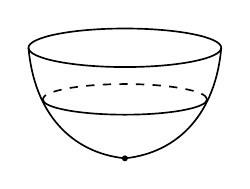
\begin{tikzpicture}[line width=0.6pt,scale=0.72]
  \draw (0,0) ellipse (1.7 and 0.34);
  \draw (-1.7,0) .. controls (-1.6,-1.15) and (-0.95,-1.85)
                 .. (0,-1.95) .. controls (0.95,-1.85) and (1.6,-1.15) .. (1.7,0);
  \draw[dashed] (1.45,-0.91) arc[start angle=0, end angle=180, x radius=1.45, y radius=0.27];
  \draw (-1.45,-0.91) arc[start angle=180, end angle=360, x radius=1.45, y radius=0.27];
  \fill (0,-1.95) circle (1.5pt);
\end{tikzpicture}
\caption{一个极小点}
\label{fig:minimum}
\end{minipage}\hfill
\begin{minipage}[b]{0.50\textwidth}
\centering

\begin{tikzpicture}[line width=0.6pt,scale=0.72]
  \draw (-2.2,0) -- (2.2,0);
  \draw (0,-2.3) -- (0,2.6);
  \draw (0,0) circle (0.6);
  \draw (0,0) circle (1.02);
  \draw (0,0) circle (1.45);
\end{tikzpicture}
\caption{\trIndex{}为~$0$ 的\trCriticalPoint}
\label{fig:critical-point-index-0}
\end{minipage}
\end{figure}

一个局部极大点是\trIndex{}为~$n$（即\trManifold{}的维数）的\trCriticalPoint。\cref{fig:critical-point-index-0}同样可以表示一个极大点附近某函数的诸\trLevelSet。

\emph{\trIndex{}~$1$。}

二元函数的\trIndex{}为~$1$ 的那些\trCriticalPoint，就是我们先前看见出现在\trTorus{}上的那些点。这些点称作“\trSaddlePoint”（saddle points）或“山口”（passes）。\cref{fig:saddle-point}解释了“鞍”这个词。“山口”这个叫法也很贴切：这幅图同样能让人联想到山口，也就是地理读本所“定义”\footnote{词典里“两山之间的狭窄通道”或“两峰之间形成通道的凹口”这类定义，也精确不到哪里去。}的“两座山峰之间的最高点”。同样地，\cref{fig:critical-point-index-1}让人想到的则是地形图上一座山口附近的等高线（level curves）。

\begin{figure}[htbp]
\begin{minipage}[b]{0.53\textwidth}
\centering
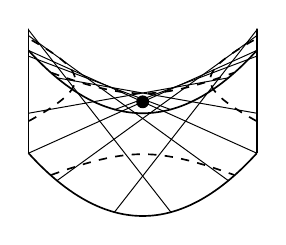
\begin{tikzpicture}[line width=0.6pt,scale=1.45]
  \begin{scope}[line width=0.35pt]
    \draw (-0.25,-0.97) -- (1,0.63);
    \draw (-0.75,-0.69) -- (1,0.58);
    \draw (-1,-0.45) -- (1,0.45);
    \draw (-1,-0.10) -- (0.75,0.21);
    \draw (-1,0.40) -- (0.25,-0.07);
    \draw (-0.25,-0.07) -- (1,0.40);
    \draw (-0.75,0.21) -- (1,-0.10);
    \draw (-1,0.45) -- (1,-0.45);
    \draw (-1,0.58) -- (0.75,-0.69);
    \draw (-1,0.63) -- (0.25,-0.97);
  \end{scope}
  \draw[dashed,domain=-0.80:0.80,samples=25,smooth]
    plot ({sqrt(\x*\x+0.35)},{0.45*\x+0.55*0.35});
  \draw[dashed,domain=-0.80:0.80,samples=25,smooth]
    plot ({-sqrt(\x*\x+0.35)},{0.45*\x+0.55*0.35});
  \draw[dashed,domain=-0.80:0.80,samples=25,smooth]
    plot (\x,{0.45*sqrt(\x*\x+0.35)-0.55*0.35});
  \draw[dashed,domain=-0.80:0.80,samples=25,smooth]
    plot (\x,{-0.45*sqrt(\x*\x+0.35)-0.55*0.35});
  \draw[domain=-1:1,samples=25,smooth] plot (\x,{0.55*\x*\x-0.10});
  \draw[domain=-1:1,samples=25,smooth] plot (\x,{0.55*\x*\x-1.00});
  \draw[domain=-1:1,samples=25,smooth] plot (1,{0.45*\x+0.55*(1-\x*\x)});
  \draw[domain=-1:1,samples=25,smooth] plot (-1,{0.45*\x+0.55*(1-\x*\x)});
  \fill (0,0) circle (1.6pt);
\end{tikzpicture}
\caption{一个\trSaddlePoint}
\label{fig:saddle-point}
\end{minipage}\hfill
\begin{minipage}[b]{0.41\textwidth}
\centering

\begin{tikzpicture}[line width=0.6pt,scale=0.9]
  \draw (-2.3,0) -- (2.3,0);
  \draw (0,-2.3) -- (0,2.3);
  \draw[domain=-2.0:2.0,smooth] plot (\x,\x);
  \draw[domain=-2.0:2.0,smooth] plot (\x,-\x);
  \draw[domain=-1.9:1.9,samples=41] plot (\x,{sqrt(\x*\x+0.30)});
  \draw[domain=-1.9:1.9,samples=41] plot (\x,{-sqrt(\x*\x+0.30)});
  \draw[domain=-1.9:1.9,samples=41] plot ({sqrt(\x*\x+0.30)},\x);
  \draw[domain=-1.9:1.9,samples=41] plot ({-sqrt(\x*\x+0.30)},\x);
  \draw[domain=-1.9:1.9,samples=41] plot (\x,{sqrt(\x*\x+0.85)});
  \draw[domain=-1.9:1.9,samples=41] plot (\x,{-sqrt(\x*\x+0.85)});
  \draw[domain=-1.9:1.9,samples=41] plot ({sqrt(\x*\x+0.85)},\x);
  \draw[domain=-1.9:1.9,samples=41] plot ({-sqrt(\x*\x+0.85)},\x);
\end{tikzpicture}
\caption{\trIndex{}为~$1$ 的\trCriticalPoint}
\label{fig:critical-point-index-1}
\end{minipage}
\end{figure}
